%%%%%%%%%%%%%%%%%%%%%%%%%%%%%%%%%%%%%%%%%%%%%%%%%%%%%%%%%%%%%%%%%%%%%% 
%
% This is a LaTeX file for an A0 poster.
% 
% template poster adapted from https://canizo.org/latex_poster
% 
% forked from  https://github.com/cvanderaa/SCB2020-Poster
%
%%%%%%%%%%%%%%%%%%%%%%%%%%%%%%%%%%%%%%%%%%%%%%%%%%%%%%%%%%%%%%%%%%%%%%

%
% Bioconductor packages for Thermal proteome profiling analysis
%
% Poster for the EuroBioC December 2020 (virtual).
%
%      Thermal proteome profiling (TPP) is a mass spectrometry-based 
%      technology which was originally developed to identify drug (off)
%      -targets on a proteome-wide scale. The assay is built on the principle
%      of the cellular thermal shift assay which is that proteins inside living
%      cells may be modulated in their thermal stability by ligand binding.
%      This can be read out by shifts of melting profiles of respective proteins. 
%      Soon after TPP was established, a first Bioconductor package `TPP` 
%      was released, which implemented function to infer ligand-protein interactions
%      using shifts of melting points. The realization that this procedure 
%      lacks sensitivity to detect proteins with e.g. very high thermal stability lead 
%      to the development of the `NPARC` package. \\
%      Further, it was realized that TPP data can also inform on protein-protein 
%      interaction dynamics. Another Bioconductor package `Rtpca` was thus implemented
%      to accomodate respective analyses. \\
%      Lastly, the experimental setup of TPP experiments was expanded to profile ligand
%      dose and temperature ranges together to improve sensitivity. To accomodate the 
%      different data structure and different required statistical analysis the package
%      `TPP2D` was created. All of these packages are presented in this poster. 
%

\documentclass{article}
% To modify the size of the page:
\usepackage[dvips,a3paper,portrait,centering,margin=0.5cm]{geometry}
% To create multiple columns
\usepackage{multicol}

\usepackage[utf8]{inputenc}
% To align images
\usepackage[export]{adjustbox}
% Use captions in minipages
\usepackage{caption}
% Math font
\usepackage{amsmath, amsthm, amsfonts}
% Include figure files.
\usepackage{graphicx}

% Coding fonts
% ------------
% For including R chunks 
\usepackage{listings} 
\lstset{
  language=R,
  basicstyle=\footnotesize\ttfamily\color{vdgray}, % the size of the fonts that are used for the code
  % sensitive=false,
  numbers=left,                   % where to put the line-numbers
  numberstyle=\tiny\color{gray},  % the style that is used for the line-numbers
  stepnumber=1,                   % the step between two line-numbers.
  numbersep=0.1cm,                % how far the line-numbers are from the code
  backgroundcolor=\color{lgray},  % choose the background color. You must add \usepackage{color}
  deletekeywords={stat},
  keywordstyle=\color{blue},      % keyword style
  stringstyle=\color{green},      % string literal style
  xleftmargin=0.5cm,
  xrightmargin=0.5cm
}
% Create command for highlighting inline code or variables
\newcommand{\hcode}[2][lgray]{{\ttfamily\color{vdgray}\colorbox{#1}{#2}}}

% Colors
% ------
\usepackage{color}
\usepackage[dvipsnames]{xcolor}
% Color panel used throughout the poster
\definecolor{lgray}{rgb}{0.9179688,0.9179688,0.9179688} % #ebebeb
\definecolor{dgray}{rgb}{0.796875,0.796875,0.796875} % #cccccc
\definecolor{vdgray}{rgb}{0.3984375,0.3984375,0.3984375} % #666666
\definecolor{coral}{rgb}{0.9960938,0.4960938,0.3125000} % #ff7f50
\definecolor{blue}{rgb}{0.4218750,0.6484375,0.8007812} % #6ca6cd
\definecolor{green}{rgb}{0.6289062, 0.8476562, 0.6054688} % #b3ba82
\definecolor{yellow}{rgb}{0.9570312,0.8671875,0.6992188} % #f5deb3

% Font
\usepackage[scaled]{helvet}
\renewcommand\familydefault{\sfdefault} 
\usepackage[T1]{fontenc}

% Bibliography
% ------------
\usepackage{url}
% Adjust space between reference items
\let\OLDthebibliography\thebibliography
\renewcommand\thebibliography[1]{
  \OLDthebibliography{#1}
  \setlength{\parskip}{0pt}
  \setlength{\itemsep}{0pt plus 0.3ex}
}
  
\pagestyle{empty}

\def\to{\rightarrow}


% ===========================================================================

\title{}
\author{}
\date{}

\begin{document}


% ---------------------------------------------------------------------------
% Banner


\begin{center}
\colorbox{lgray}{
  %\begin{minipage}{3.7cm}
  %  \includegraphics[width=1.2\linewidth]{}
  %\end{minipage}
  %&
  \begin{minipage}{.865\textwidth}
    %\begin{center}
      % Title 
      \vspace{0.4cm}
      \huge 
      %\hspace{1cm}
      \noindent
      \textbf{Bioconductor packages for analysis of Thermal Proteome Profiling data} \\
      \vspace{0.05cm} \\
      % Authors
      \Large Nils Kurzawa$^{1,*}$, Dorothee Childs$^{1,2}$, Holger Franken$^2$, Mikhail M. Savitski$^1$ \& Wolfgang Huber$^1$ \\
      \vspace{0.05cm} \\
      % Affiliation
      \Large \textit{$^1$Genome Biology Unit, European Molecular Biology Laboratory} \\
      \Large \textit{$^2$Cellzome GmbH, GlaxoSmithKline} \\
      \vspace{0.05cm} \\
      % email
      %\vspace{0.4cm}
      \normalsize $^*$contact: nils.kurzawa@embl.de \\
    %\end{center}
  \end{minipage}
  %&
  \begin{minipage}{3.7cm}
      \includegraphics[width=1.2\linewidth, right]{} \\
      \vspace{0.5cm}
      
\includegraphics[width=1.1\linewidth, right]{figs/embl_logo.png}
  \end{minipage}
}
\end{center}


% ---------------------------------------------------------------------------
% Summary + conclusion
\noindent
% Summary
\colorbox{green}{
  \noindent
  \begin{minipage}[t]{\textwidth}
    \vspace{.15cm}
    %\section*{\huge Summary}
    \large 
      Thermal proteome profiling (TPP) is a mass spectrometry-based 
      technology which was originally developed to identify drug (off)
      -targets on a proteome-wide scale. The assay is built on the principle
      of the cellular thermal shift assay which is that proteins inside living
      cells may be modulated in their thermal stability by ligand binding.
      This can be read out by shifts of melting profiles of respective proteins. 
      Soon after TPP was established, a first Bioconductor package \hcode{TPP} 
      was released, which implemented a method to infer ligand-protein interactions
      using shifts of melting points. The realization that this procedure 
      lacks sensitivity to detect proteins with e.g. very high thermal stability lead 
      to the development of the \hcode{NPARC} package. 
      Further, it was realized that TPP data can also inform on protein-protein 
      interaction (PPI) dynamics. Another Bioconductor package \hcode{Rtpca} was thus implemented
      to accomodate respective analyses. 
      Lastly, the experimental setup of TPP experiments was expanded to profile ligand
      dose and temperature ranges together to improve sensitivity. To accomodate the 
      different data structure and different required statistical analysis the package
      \hcode{TPP2D} was created. Here, the different functionalities of these packages are presented. 
      
    \vspace{0.1cm}
  \end{minipage}
}
%\hspace{0.37cm}
%% Conclusion
%\noindent
%\colorbox{green}{
%  \begin{minipage}[t]{13.6cm}
%    \vspace{.2cm}
%    \section*{\huge Take home message}
%    \large
%      The amount of available MS-based SCP data is rapidly increasing 
%      and so is the need for dedicated analysis software. We offer 
%      two R/Bioconductor packages. The first package, \hcode[yellow]
%      {scpdata}, disseminates curated SCP data sets for method 
%      development and benchmarking. The second package, \hcode[yellow]
%      {scp}, implements functions to streamline the analysis of SCP 
%      data. This work provides the ground for reproducible and 
%      rigorous development and benchmarking of new state-of-the-art 
%      methods.
%    \vspace{0.15cm}
% \end{minipage}
%}
\vspace{-1cm}


% ---------------------------------------------------------------------------
% Create a 2 column layout
\setlength{\columnsep}{0.5cm}
\begin{multicols}{2}

% ---------------------------------------------------------------------------
% The TPP technology
\noindent
\begin{minipage}[t]{\linewidth}
  \vspace{0.5cm}
  \section*{\huge Thermal Proteome Profiling (TPP)}
  \subsection*{TPP over a temperature range (TPP-TR) \cite{savitski_2014}}
  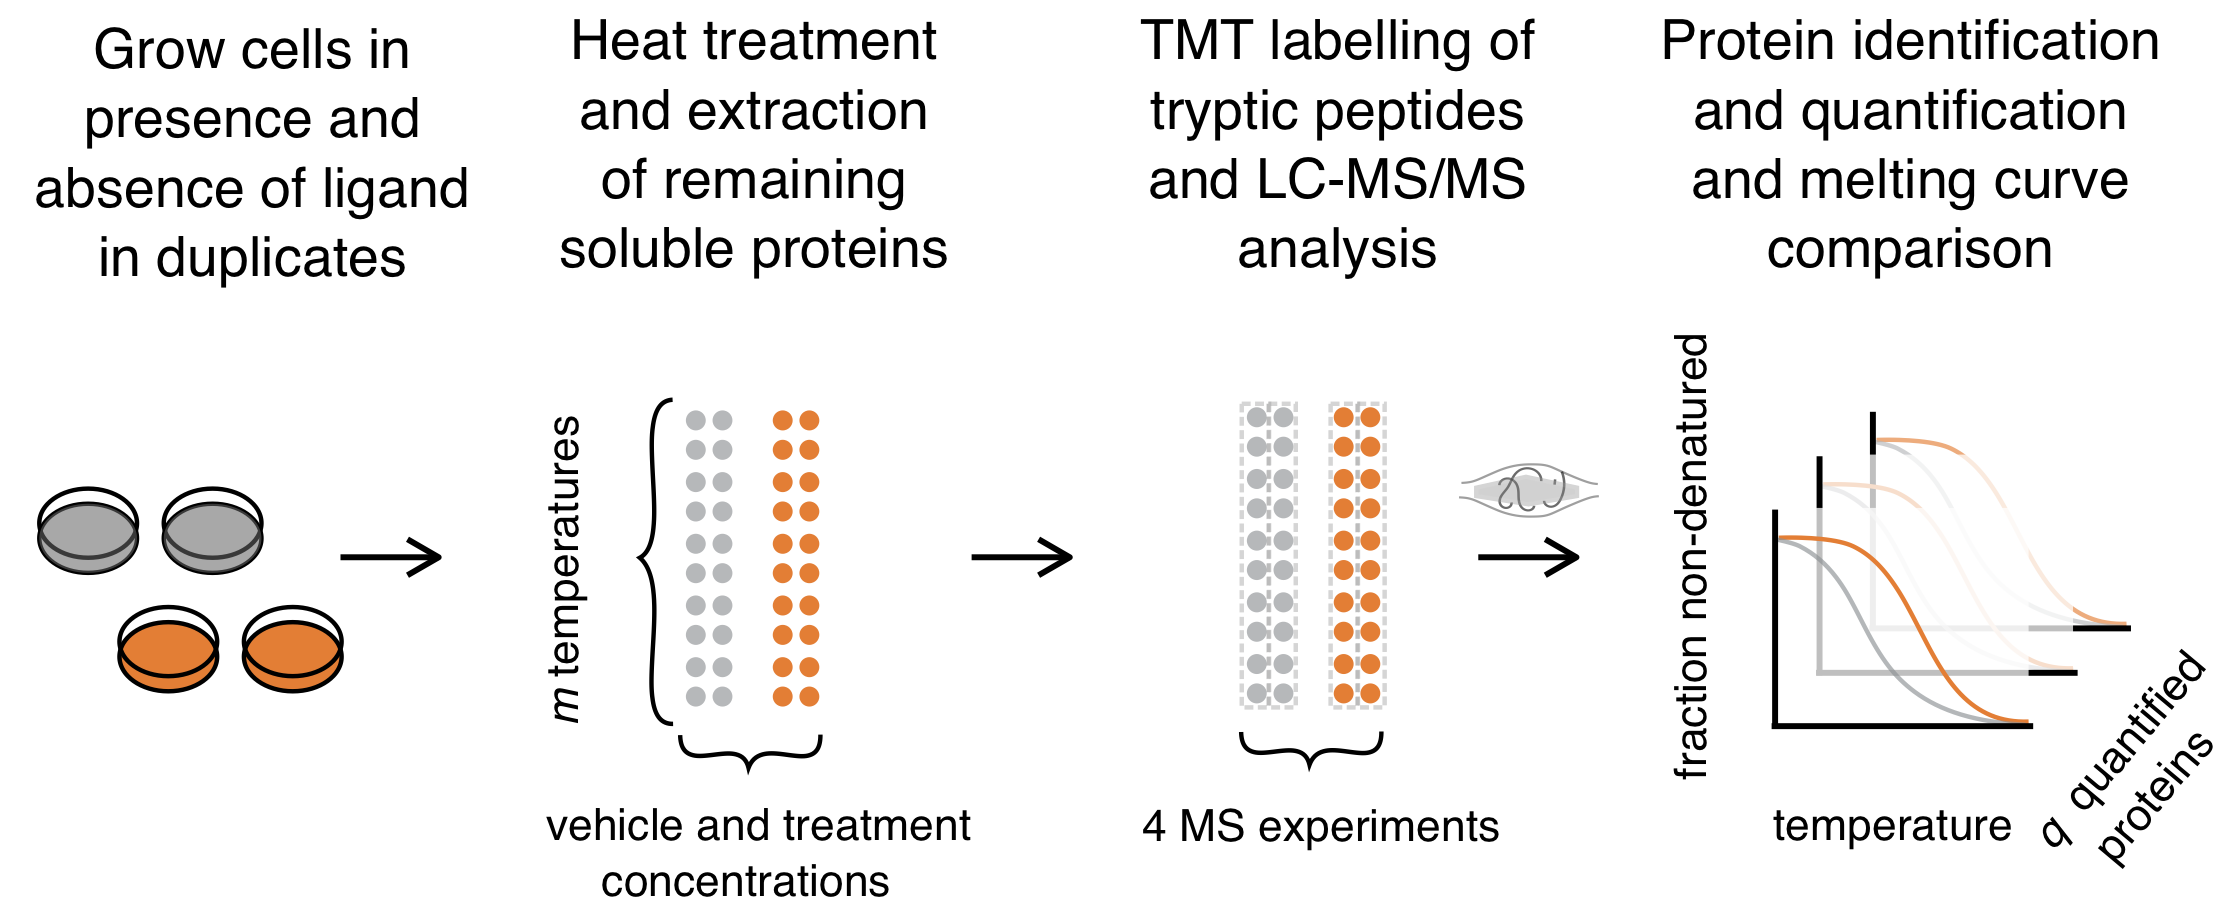
\includegraphics[width=\linewidth]{figs/tpp-tr_schematic.png}
  \subsection*{Ligand dose and temperature range TPP (2D-TPP) \cite{becher_2016}}
  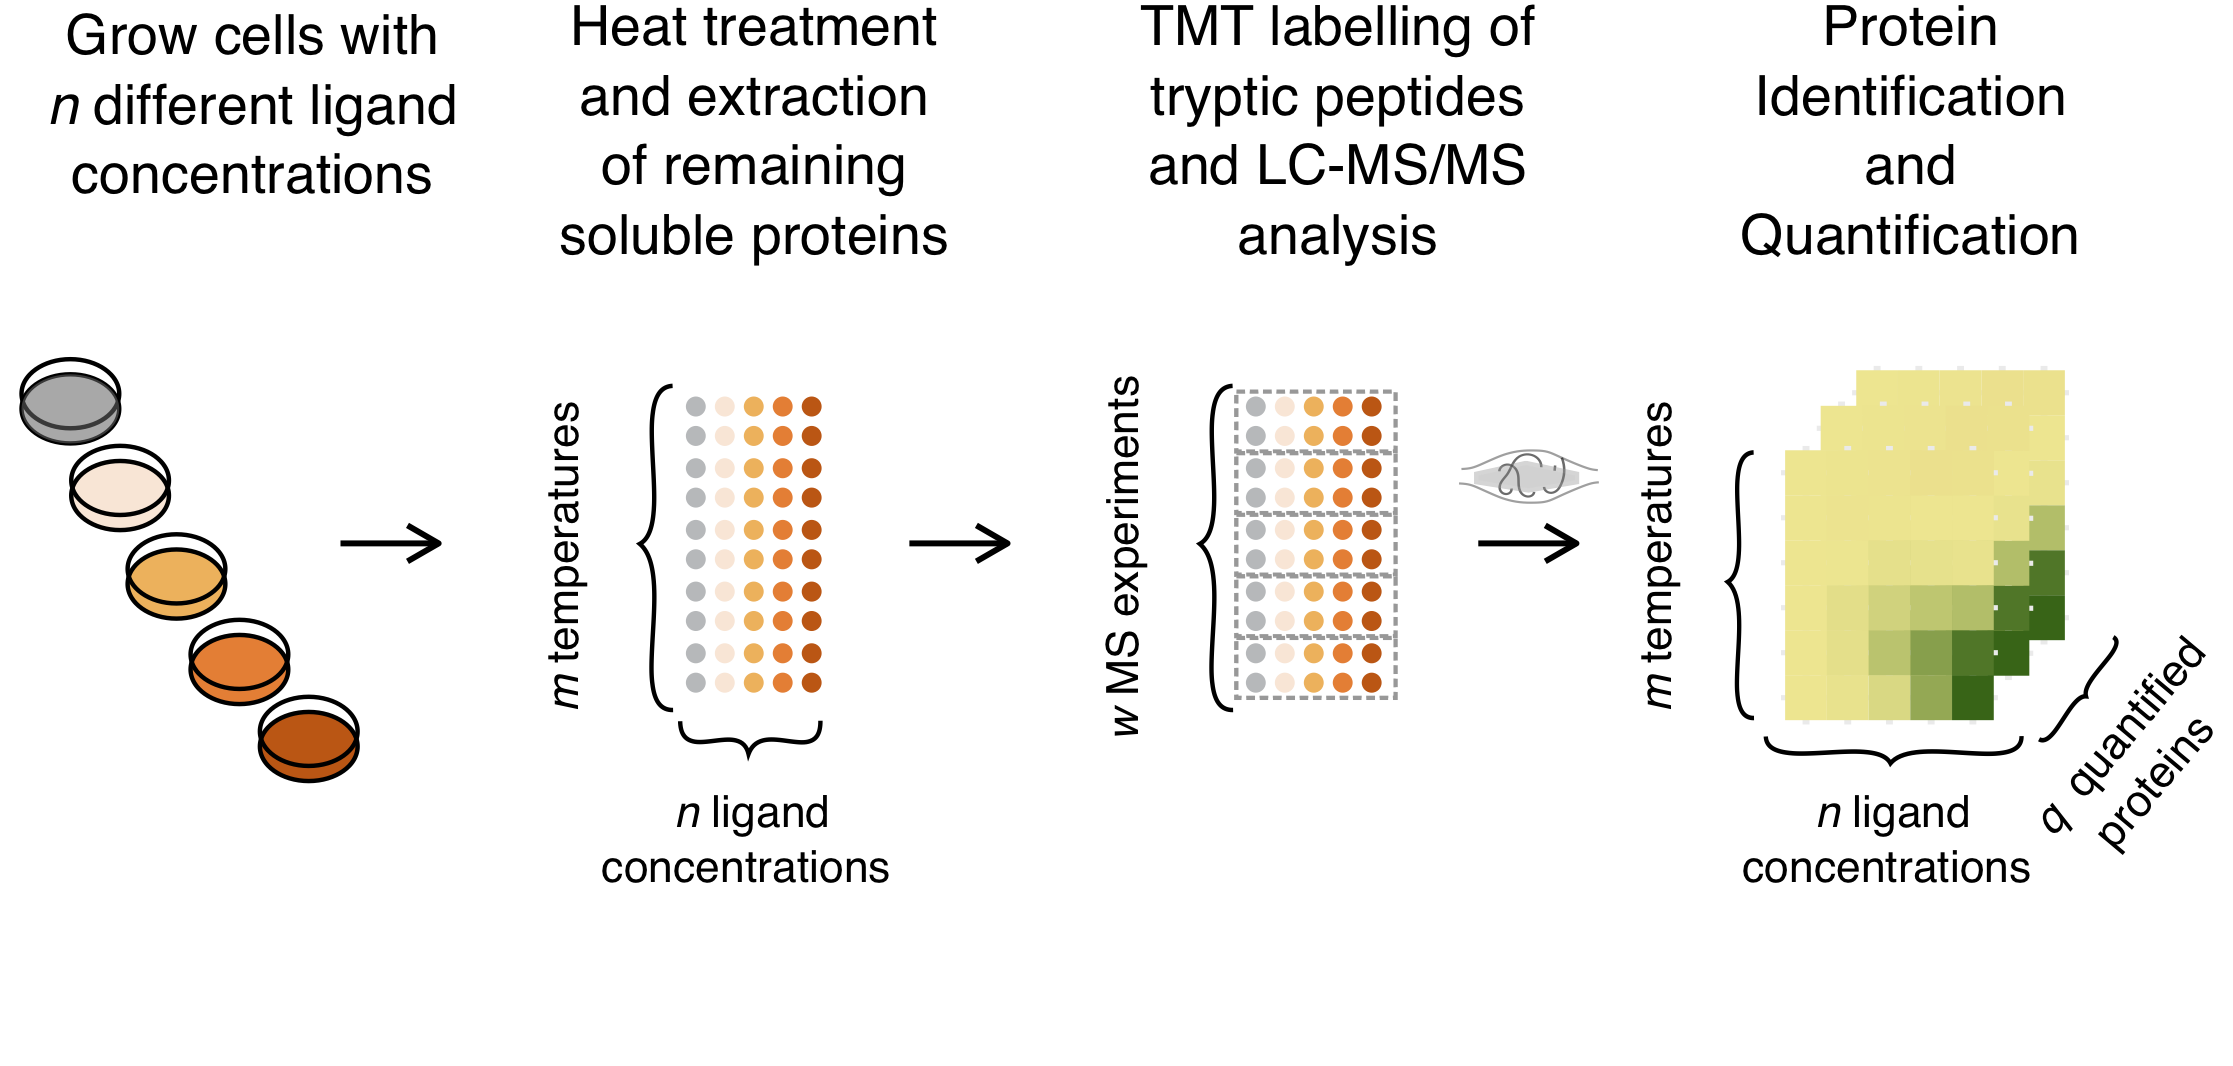
\includegraphics[width=\linewidth]{figs/2d-tpp_schematic.png}
%\end{minipage}

%\vspace{-2cm}
% ---------------------------------------------------------------------------
% TPP 
%\noindent
%\begin{minipage}[t]{\linewidth}
 % \vspace{0.55cm}
  \section*{\huge TPP-TR analysis with \hcode{TPP} \cite{franken_2015}}
  Melting point-centric data analysis.

  \begin{minipage}{0.6\linewidth}
  %\begin{center}
  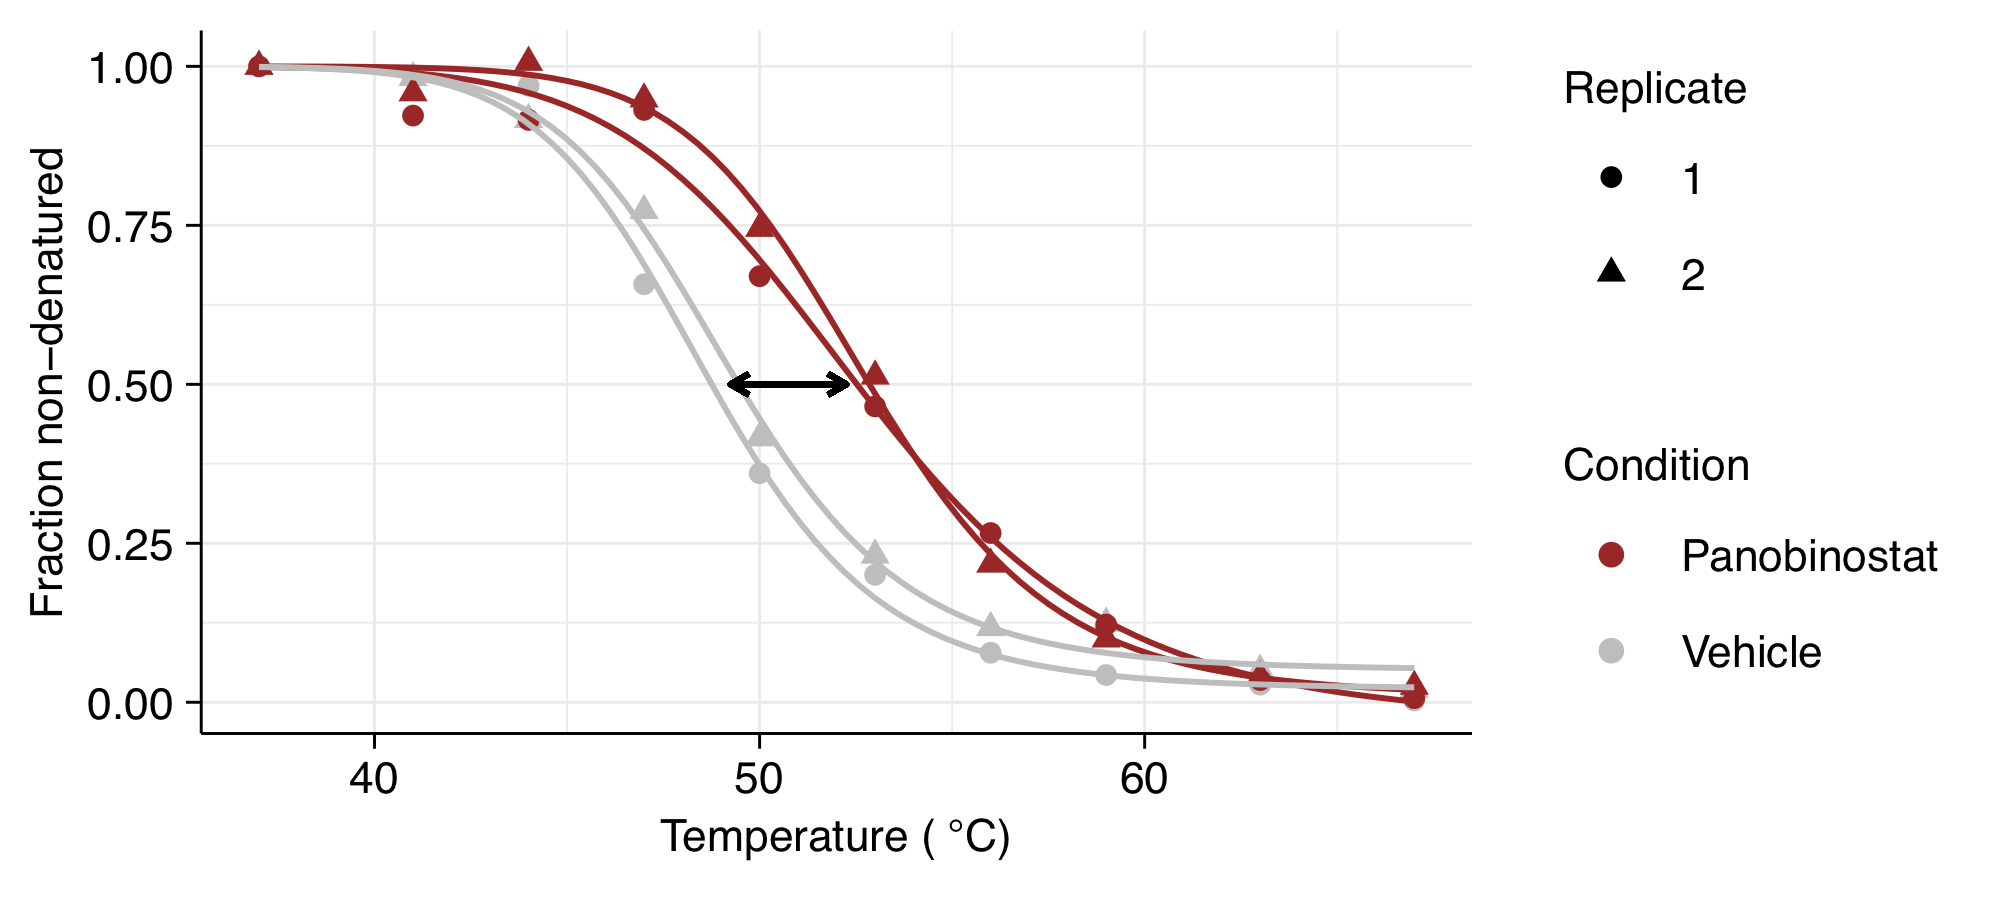
\includegraphics[width=\linewidth]{figs/tpp-tr_example.png}
  %\end{center}
  \end{minipage}%
  \begin{minipage}{0.4\linewidth}

  \textbf{Features of the \hcode{TPP} package}:

  \begin{itemize}

  \item TPP-TR data import into ExpressionSet structure
  \item data normalization and melting curve fitting, detection of melting point shifts
  \item analysis of isothermal concentartion range TPP experiments
  
  \end{itemize}
  \end{minipage}
%\end{minipage}

% ---------------------------------------------------------------------------
% NPARC
%\noindent
%\begin{minipage}[ht]{\linewidth}
%  \vspace{0.55cm}
  \section*{\huge TPP-TR analysis with \hcode{NPARC} \cite{childs_2019}}
  Nonparametric analysis of response curves comparing exploiting all measurements.  

  \begin{minipage}{0.6\linewidth}
  %\begin{center}
  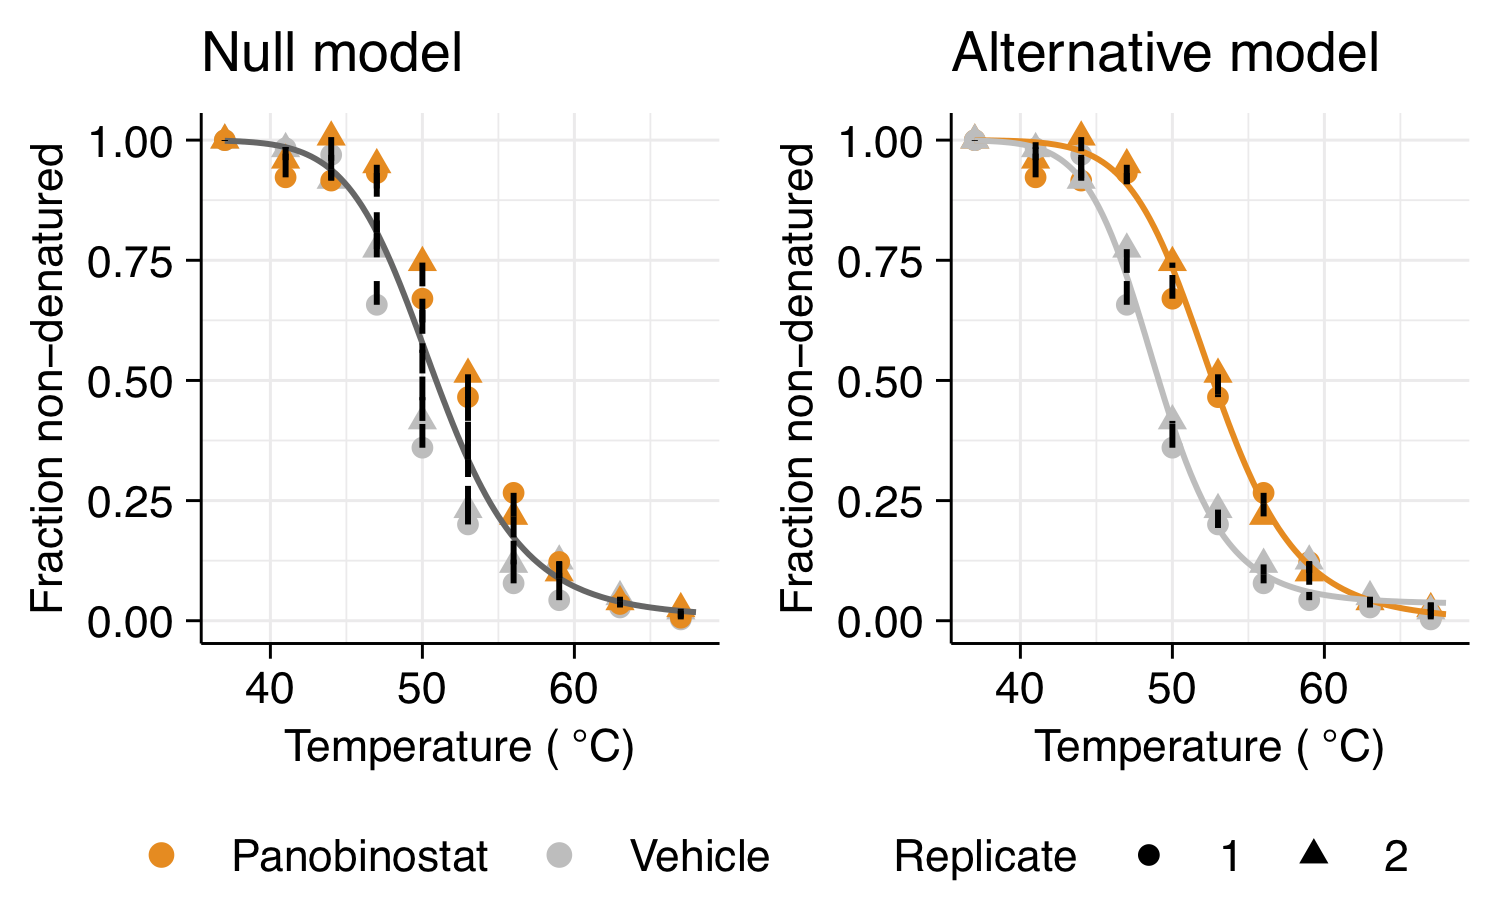
\includegraphics[width=\linewidth]{figs/nparc-tr_example_new.png}
  \end{minipage}%
  \begin{minipage}{0.4\linewidth}
  %\end{center}
  \textbf{Features of the \hcode{NPARC} package}:
% 
  \begin{itemize}
%
  \item light-weight package for performing sensitive differential melting curve analysis
  \item nested model comparison: one sigmoidal across conditions vs. sigmoidals per condition
  \item $F$-statistic based on explained variance of each model
  \item method for calibration of retrieved $F$-statistics
%
  \end{itemize}
  \end{minipage}
\end{minipage}


% ---------------------------------------------------------------------------
% Rtpca
\noindent
\begin{minipage}[t]{\linewidth}
  \vspace{0.55cm}
  \section*{\huge Detecting differential PPIs with \hcode{Rtpca} \cite{kurzawa_2020}}
  Detecting (differential) thermal co-aggregation of interacting proteins.
  \begin{center}
  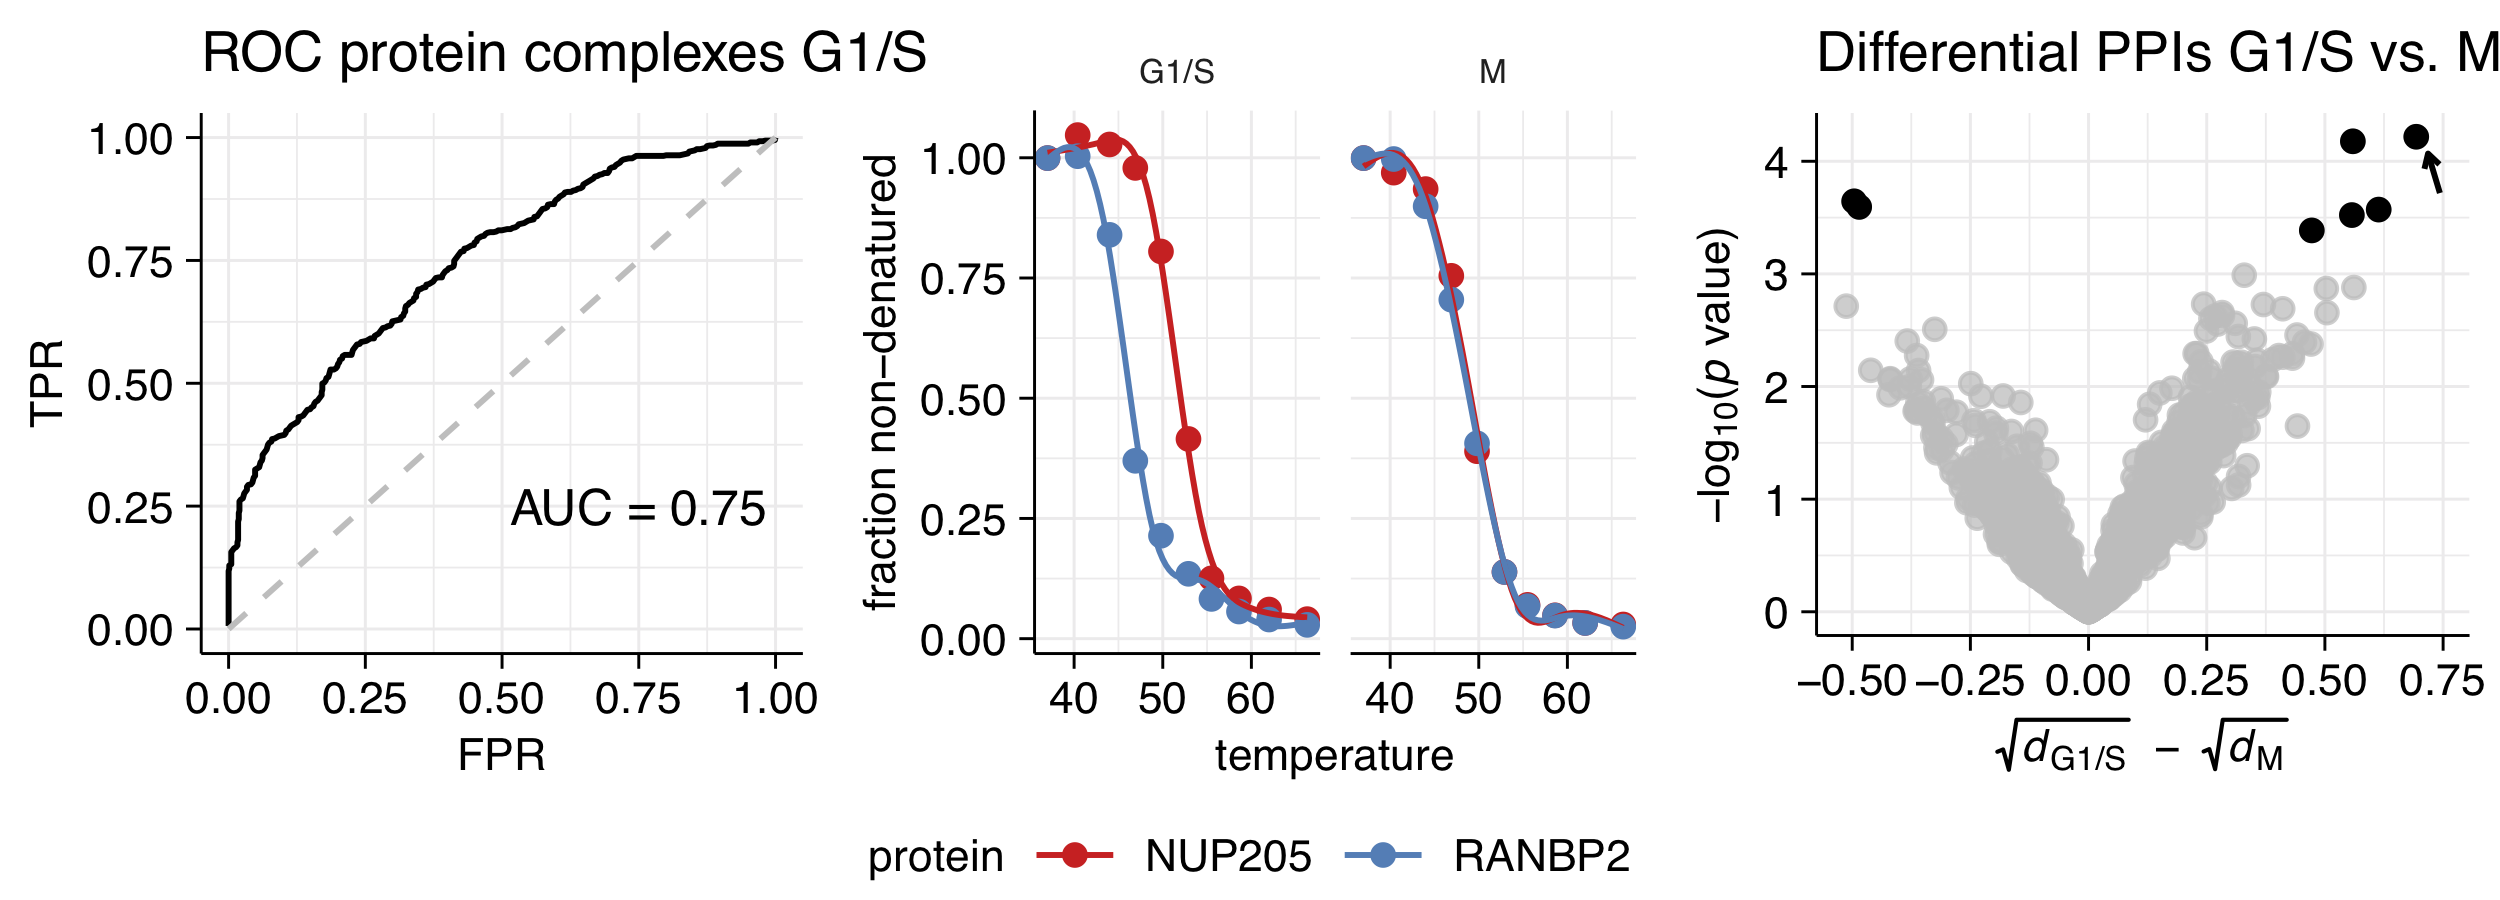
\includegraphics[width=\linewidth]{figs/rtpca-tr_example.png}
  \end{center}
  \textbf{Features of the \hcode{Rtpca} package}:
  \begin{itemize}
%
  \item test for co-aggregation of annotated protein-protein interactors (PPI), compute receiver operating characteristics (ROC)
  \item perform differential testing to find changes in PPIs between different conditions
%
  \end{itemize}
\end{minipage}



% ---------------------------------------------------------------------------
% TPP2D
\noindent
\begin{minipage}[t]{\linewidth}
  \vspace{0.55cm}
  \section*{\huge 2D-TPP data analysis with \hcode{TPP2D} \cite{kurzawa_2020a}}
  FDR-controlled detection of ligand-protein interactions from 2D thermal profiles.
  
  \begin{center}
  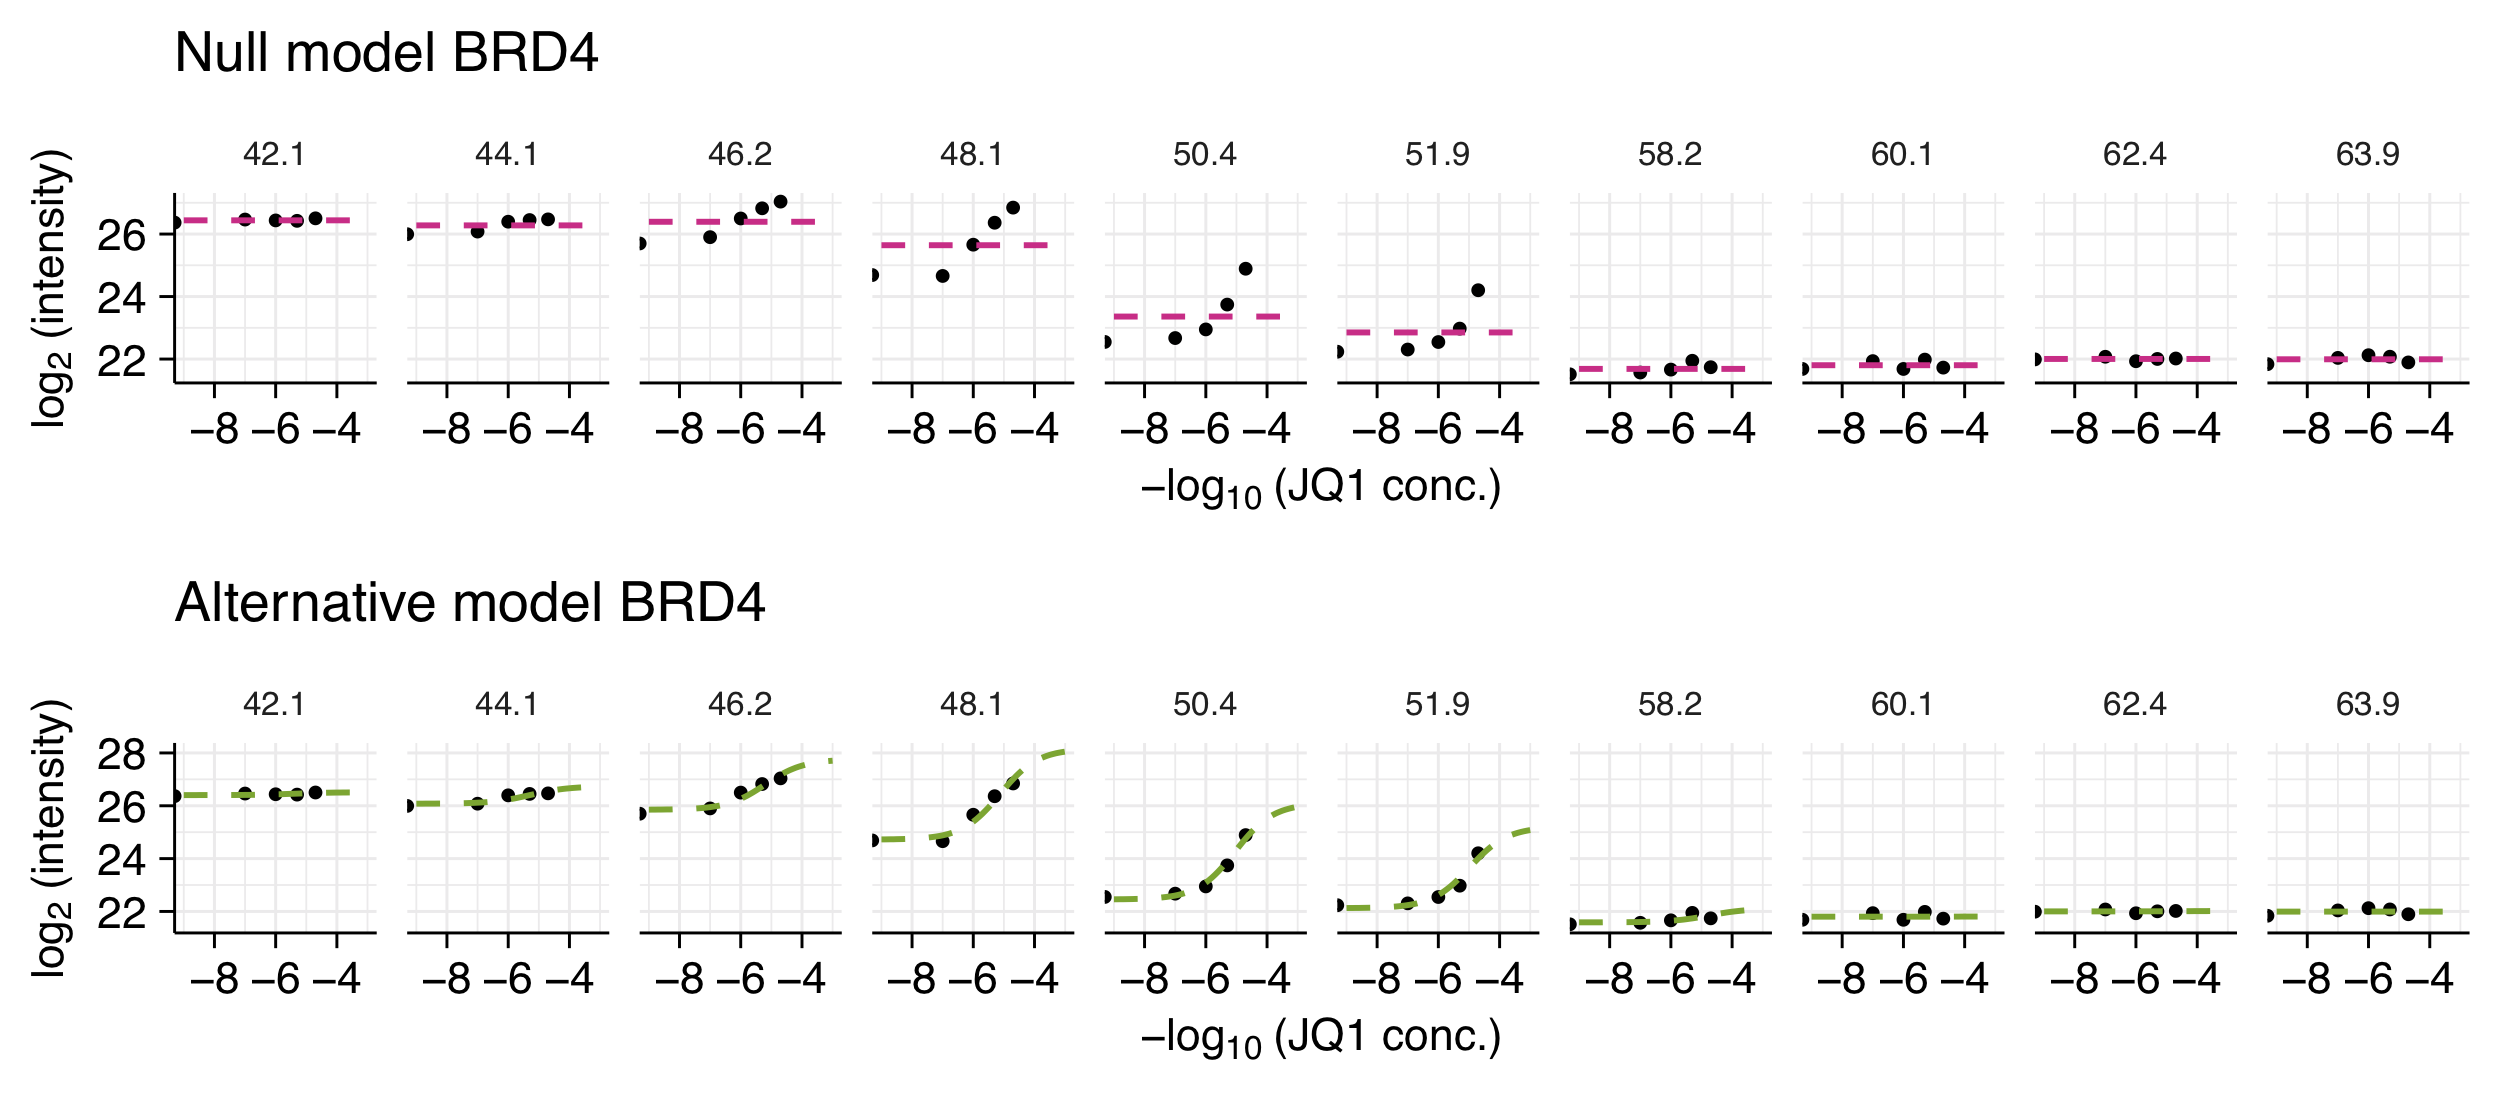
\includegraphics[width=\linewidth]{figs/tpp2d_example.png}
  \end{center}

  \begin{minipage}{0.4\linewidth}
  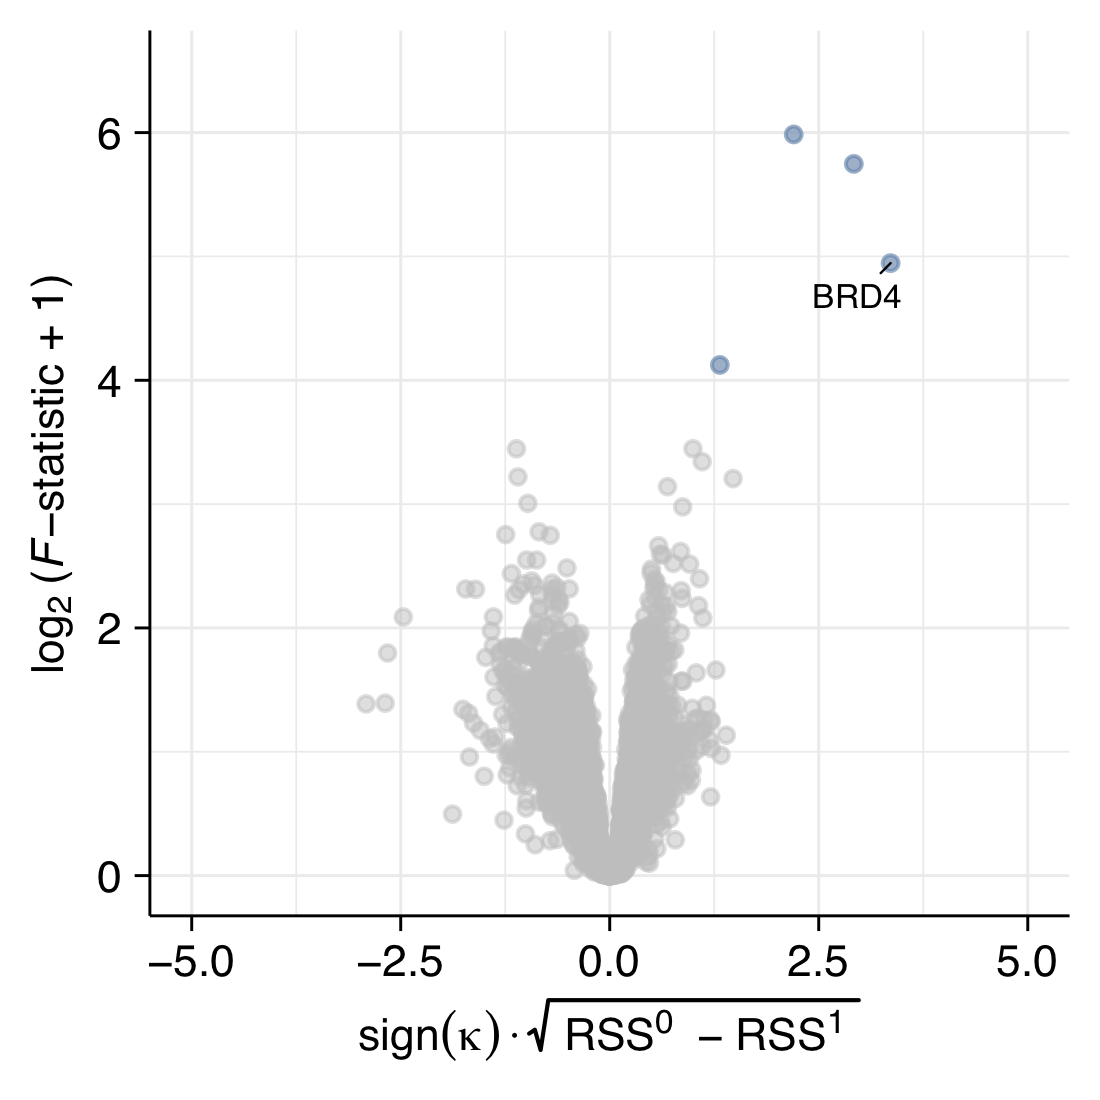
\includegraphics[width=\linewidth]{figs/tpp2d_volcano.png}
  \end{minipage}%
  \begin{minipage}{0.6\linewidth}
  \textbf{Features of the \hcode{TPP2D} package}:
% 
  \begin{itemize}
%
  \item hypothesis test on curves: intercept model vs. dose-response model contrained across temperatures
  \item bootstrapping approach to calibrate $F$-statistic in terms of false discovery-rate (FDR)
  \item several functions for data visualization
%
  \end{itemize}
  \end{minipage}
  
\end{minipage}

% ---------------------------------------------------------------------------
% References
\scriptsize
\bibliography{ref.bib} 
\bibliographystyle{ieeetr}

% ---------------------------------------------------------------------------
% Additional notes
\noindent
This work was funded by EMBL and GSK. The poster is available at {\color{blue}
{https://github.com/nkurzaw/EuroBioc2020Poster}}.

% ---------------------------------------------------------------------------
% End of poster
\end{multicols}
\end{document}
